\documentclass[a4paper,11pt]{article}
\usepackage[american]{babel}
\usepackage[utf8]{inputenc}
\usepackage{geometry}
\usepackage[ruled,vlined]{algorithm2e}
 \usepackage{algpseudocode}
\usepackage{booktabs}  
\usepackage{graphicx} 
\usepackage{listings}
\usepackage{ragged2e}
\usepackage{caption}
\usepackage{subcaption}
\usepackage{float}
\usepackage{syntax}
\usepackage[dvipsnames]{xcolor}
\usepackage{listings}

\lstdefinelanguage{Kotlin}{
  comment=[l]{//},
  commentstyle={\color{gray}\ttfamily},
  emph={delegate, filter, first, firstOrNull, forEach, lazy, map, mapNotNull, println, return@},
  emphstyle={\color{OrangeRed}},
  identifierstyle=\color{black},
  keywords={abstract, actual, as, as?, break, by, class, companion, continue, data, do, dynamic, else, enum, expect, false, final, for, fun, get, if, import, in, interface, internal, is, null, object, override, package, private, public, return, set, super, suspend, this, throw, true, try, typealias, val, var, vararg, when, where, while},
  keywordstyle={\color{NavyBlue}\bfseries},
  morecomment=[s]{/*}{*/},
  morestring=[b]",
  morestring=[s]{"""*}{*"""},
  ndkeywords={@Deprecated, @JvmField, @JvmName, @JvmOverloads, @JvmStatic, @JvmSynthetic, Array, Byte, Double, Float, Int, Integer, Iterable, Long, Runnable, Short, String},
  ndkeywordstyle={\color{BurntOrange}\bfseries},
  sensitive=true,
  stringstyle={\color{ForestGreen}\ttfamily},
}
\lstset{%
backgroundcolor=\color{cyan!10},
basicstyle=\ttfamily,
numbers=left,numberstyle=\scriptsize
}

\usepackage[wby]{callouts}
\begin{document}
\section{Fragment Comedores}

\vspace{5 mm}

El objetivo de este fragment es facilitar al usuario que pueda ver el menú semanal que ofrece la UGR en todos sus comedores.

Para ello vamos a hacer uso principalmente de una \textbf{WebView} que va a cargar el pdf \textbf{http://scu.ugr.es/?theme=pdf} apoyándonos en Google Drive. 

\vspace{5 mm}

También vamos a hacer uso de una \textbf{ProgressBar} que nos indicará como va el proceso de carga de la url. Vemos necesario usarla porque si no parece que la pantalla no está cargando y el fragment no funciona bien.

\vspace{5 mm}

A continuación vamos a ver las variables y los métodos que forman este fragment, y que hace cada uno. 

\vspace{5 mm}

\subsection{Variables}

\vspace{5 mm}

\begin{itemize}

\item{lateinit var webview: WebView}
\item{lateinit var barra: ProgressBar}
\item{lateinit var pdf: String}

\end{itemize}

Las dos primeras variables son la propia \textbf{WebView} y la \textbf{ProgressBar} de las que he hablado antes. Ambas serán inicializadas en el método \textbf{OnCreateView} usando los id del layout. 
La tercera variable corresponde al string que guardará la url de los comedores universitarios y que pasaremos como parámetro al método \textbf{loadUrl} de la WebView.

\newpage

\subsection{Métodos}

\vspace{5 mm}

Los métodos que voy a explicar a continuación son:

\begin{itemize}
\item{onCreateView}
\end{itemize}

\vspace{5 mm}

\subsubsection{Método OnCreateView}

\vspace{5 mm}

Este método comienza inicializando las variables \textbf{webview} y \textbf{barra} explicadas anteriormente mediante \textbf{findViewById} y pasándole la Id del layout.

También le asignamos a \textbf{pdf} la url de los comedores universitarios.

\vspace{5 mm}

Una vez hecho esto, vamos a configurar la \textbf{WebView} de tal forma que pueda usar JavaScript 

\vspace{5 mm}


\begin{lstlisting}[language=Kotlin]
webview.settings.javaScriptEnabled = true
\end{lstlisting}

\vspace{5 mm}


y que el usuario pueda usar gestos para acercar y alejar la WebView a su antojo 

\vspace{5 mm}


\begin{lstlisting}[language=Kotlin]
webview.settings.setSupportZoom(true)
webview.settings.builtInZoomControls = true
\end{lstlisting}

\vspace{5 mm}

También haremos invisible la webview nada más iniciar el fragment para que lo que se vea sea la \textbf{ProgressBar} cargando.

\vspace{5 mm}

Ahora lo que nos quedaría sería modificar dos objetos internos de nuestra \textbf{WebView}. El primero sería su objeto \textbf{WebChromeClient()}. Este objeto tiene un método llamado \textbf{onProgressChanged} que nos permite ver cómo va el progreso de carga de la WebView, es por esto que lo usaremos para ocultar la webview si el progreso es menor a 100, al mismo tiempo que vamos mostrando como avanza la progressBar. Cuando el progreso llegue a 100, mostraremos la WebView y ocultaremos la ProgressBar.

\vspace{5 mm}

El otro objeto es el \textbf{WebViewClient()}, el cual tiene un método llamado \textbf{shouldOverrideUrlLoading} y que tiene como parámetro una \textbf{request} que le pasaremos a \textbf{webView.loadUrl(request)}. De esta forma, cada vez que hagamos \textit{"tap"} sobre algún enlace, se recargará la WebView mostrando el enlace.

\vspace{5 mm}

Finalmente nos quedaría mostrar la URL de los comedores universitarios mediante el método \textbf{loadUrl} de nuestra WebView.

\newpage

\begin{figure}[H]
\begin{subfigure}{0.5\textwidth}
  \centering
  % include first image
  \includegraphics[width=1\linewidth]{imagenes/progressBar.jpeg}  
  \caption{Barra de progreso}
  \label{fig:sub-first}
\end{subfigure}
\begin{subfigure}{0.5\textwidth}
  \centering
  % include second image
  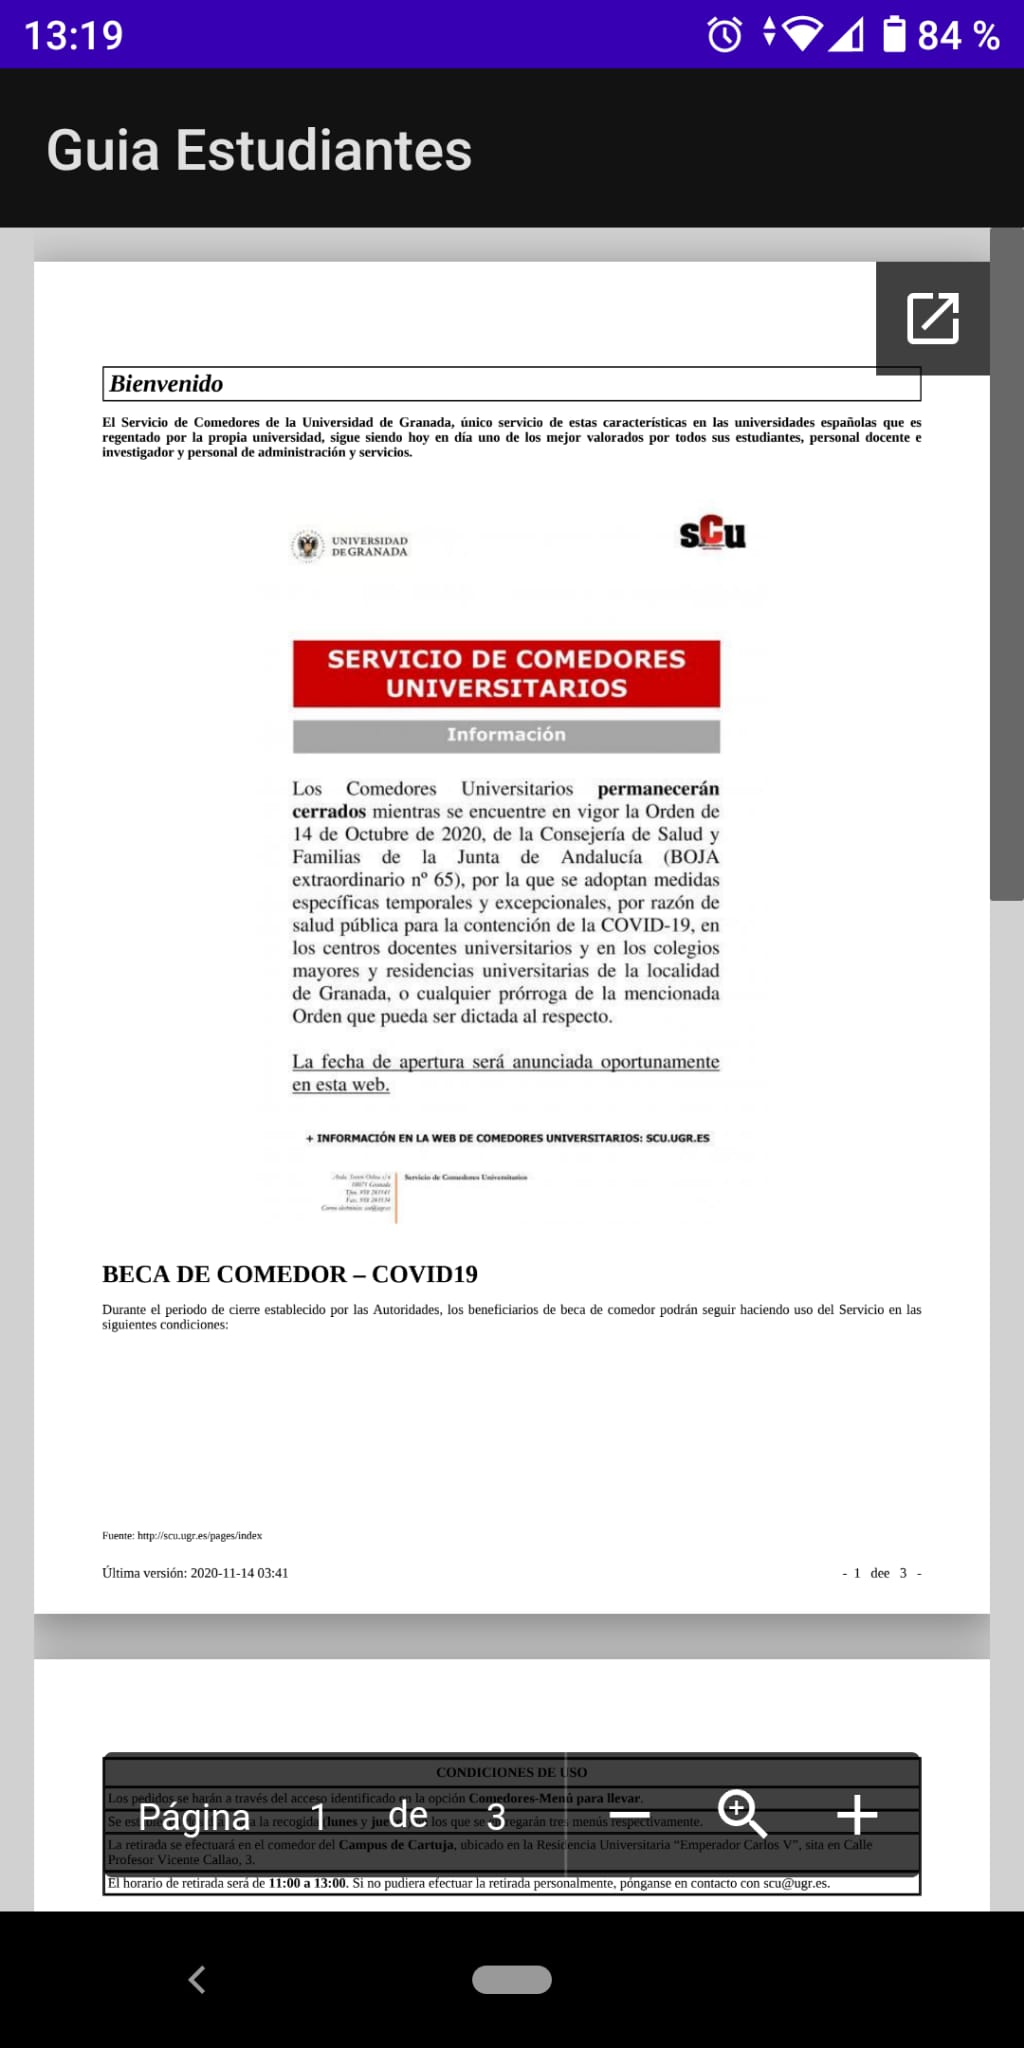
\includegraphics[width=1\linewidth]{imagenes/comedores.jpeg}  
  \caption{PDF comedores cargado}
  \label{fig:sub-second}
\end{subfigure}
\end{figure}

\end{document}